\chapter{Klassediagram}
For at illustrere modellaget i vores MVC-mønster, har vi produceret et klassediagram (se \myref{diagram:klassediagram} nedenfor) i UML, der simplificerer strukturen. 
Det skal bemærkes, at klasserne og felterne er på dansk i diagrammet, og på engelsk i selve koden af programmet. \fxfatal{Der er ingen adgangsting på dette, private, protected, public etc. Er det bevist? Derudover er det ikke klart hvilken datatype hvert felt er, også om det er en liste eller ej. - Troels}

\begin{figure}[H]
\centering
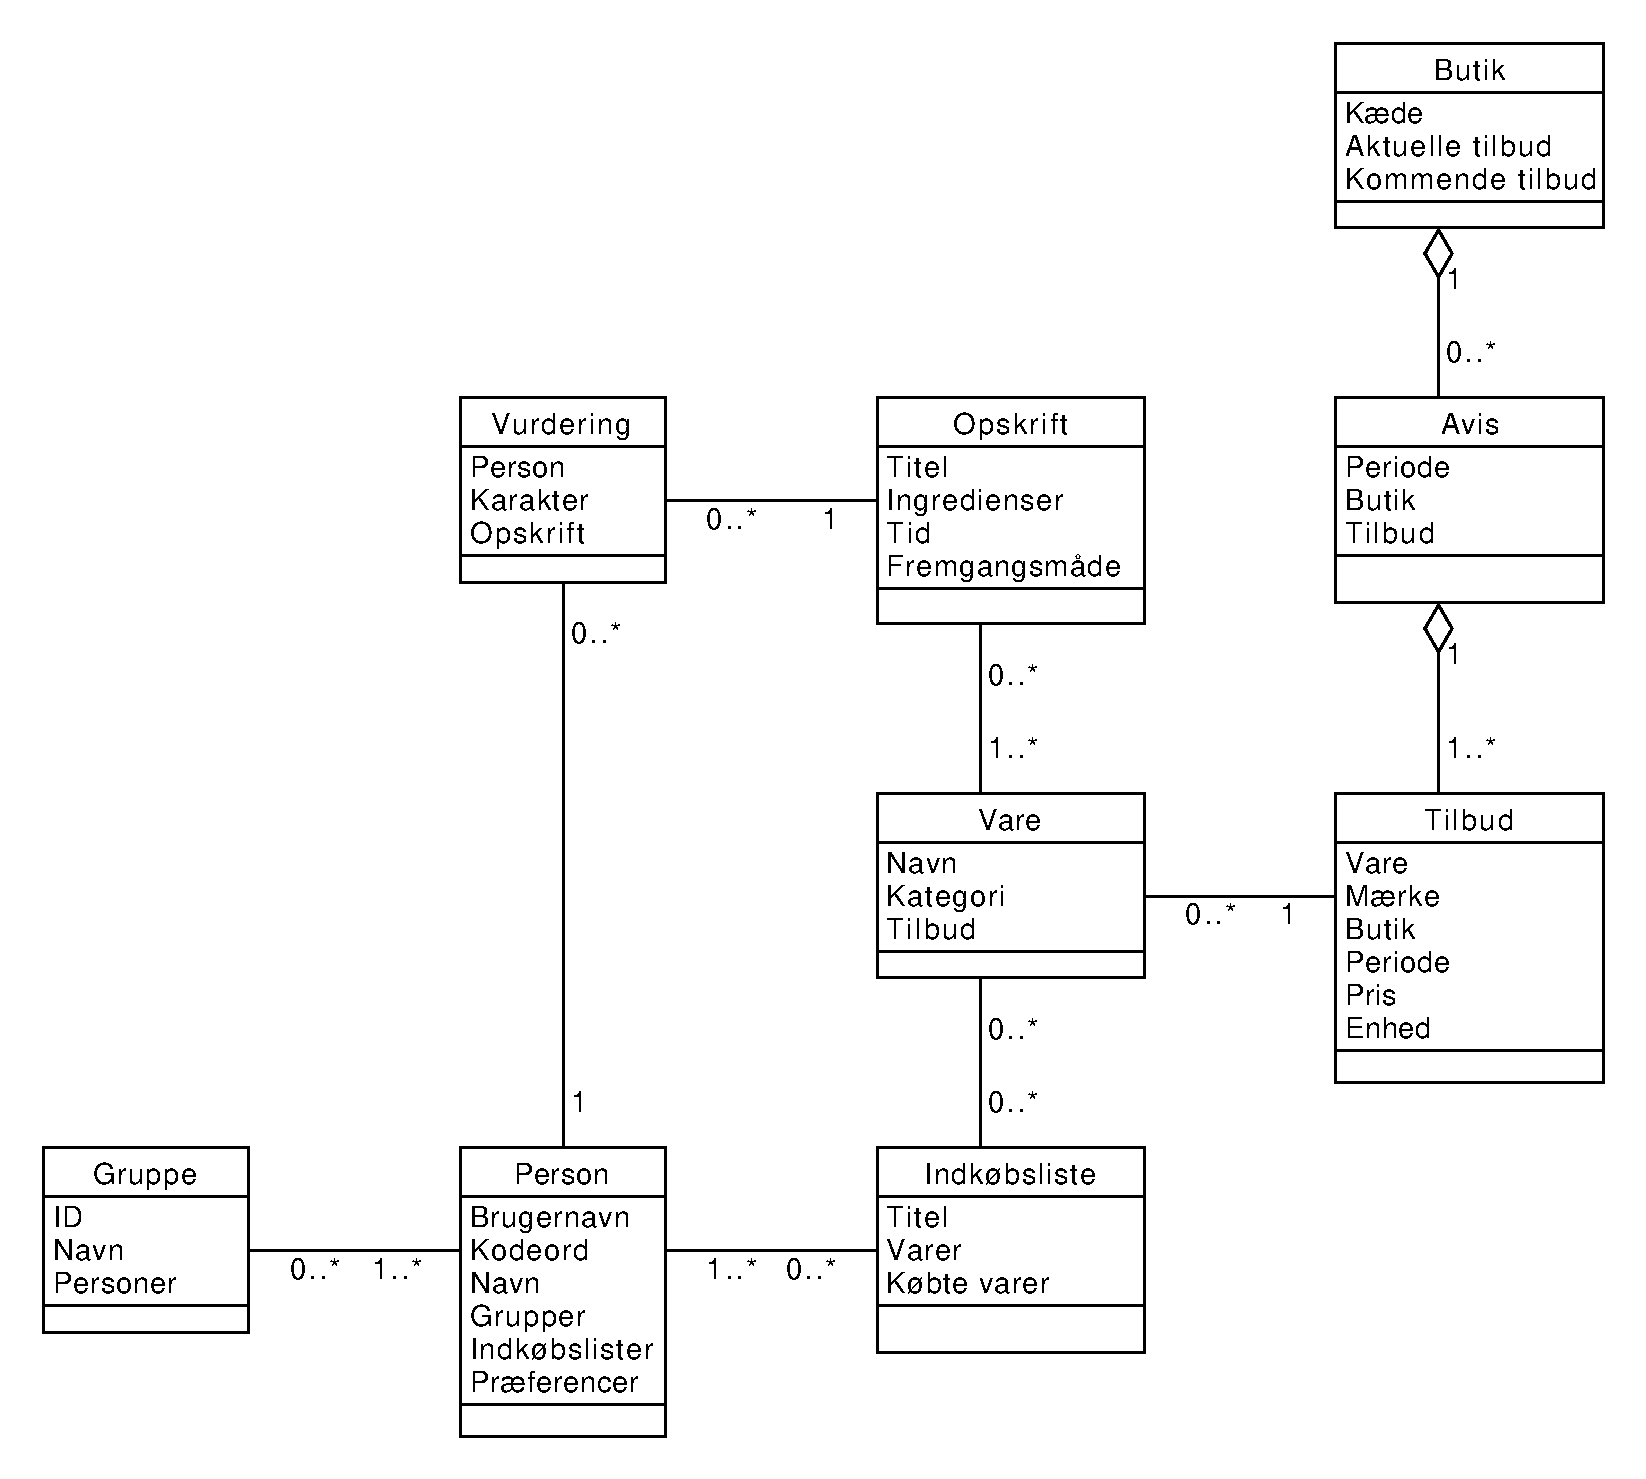
\includegraphics[width=0.8\linewidth]{/Diagrams/klassediagram_model_expanded_implemented.pdf}
\caption{UML klassediagram for modellaget i MVC-mønsteret}\label{diagram:klassediagram}
\end{figure}

\section{Klasserne}
Vi vil gennemgå klasserne, der optræder i klassediagrammet, og beskrive deres relatoner samt de felter de indeholder.

\subsection{Person}
Person-klassen i modellen, er den der holder styr på brugeren og dennes basale atributter - herunder brugernavn, kodeord og kaldenavn. 
Ydermere er det vigtigt, at objektet kan indeholde informationer om personens madpræferencer og vurderinger af opskrifter; dette er med til at give person-klassen en mere intim vinket, og så at sige bedre afspejle den virkelige person, samt fungere som grundlag for anbefaling af opskrifter. 
Det er naturligvis også vigtigt for et program, der omhandler bl.a. indkøbslister, at holde styr på en persons indkøbslister og lignende. 
Til dette har person-klassen to felter der hedder henholdsvis, grupper og indkøbslister. 
Begge felter er lister\fxfatal{Som nævnt tidligere er dette ikke klart fra diagrammet. - Troels}, der holder styr på personens relationer til netop grupper og indkøbslister - En person kan altså have relationer til flere grupper og flere indkøbslister, hvilket også kan ses ud fra de indtegnede relationer i klassediagrammet.

\subsection{Gruppe}
Klassen ``Gruppe'', bruges i programmet som en hjælpe-klasse, der binder flere personer sammen om en eller flere indkøbslister. 
På den måde er det, gennem denne klasse, muligt at dele indkøbslister med andre personer; 
Man kunne forestille sig en situation i en husstand, hvor flere personer handler ind, og det derfor ville være fordelagtigt, hvis man kunne være fælles om en indkøbsliste.
Gruppe-klassen indeholder to atributter der muliggører identifikation: Et ID, der skal være unikt for den enkelte gruppe, så programmet kan skelne mellem grupper; og er navn, der kan sætter af personer i gruppen, så netop personerne kan se forskel på de grupper de er med i. 
Herudover har klassen to lister, der hver især holder styr på relationerne til henholdsvis personer i gruppen og indkøbslister delt i gruppen.
En gruppe har relationer til en eller flere personer, og kan godt eksistere uden indkøbslister.

\subsection{Indkøbsliste}
Indkøbslister repræsenteres i systemet som klassen ''Indkøbsliste'', og indeholder ID, titel og to lister med varer. 
ID'et garanterer, at alle indkøbslister er unikke og kan skelnes fra hinanden på systemsiden - akkurat ligesom det gøres i Gruppe-klassen. 
Også i Indkøbsliste-klassen har vi et titel felt, så brugeren også kan navigere mellem forskellige instanser.
De to lister af varer, holder styr på henholdsvis; varer som bliver tilføjet til listen, og varer som har været tilføjet men er blever markeret som købt. 
Der er således kun styr på ''overstregede'' varer - altså dem der er købt, og ikke varer som bliver slettet fra listen.
En indkøbsliste kan godt eksisterer uden varer, idet brugeren skal kunne oprette lister, inden der er taget stilling til, hvilke varer der skal bruges.
Indkøbsliste har kun relation til en gruppe, men kan godt have relationer til flere personer.

\subsection{Vare}
Vare-klassen indeholder tre felter: Et navn på varen, som er generisk, for eksempel ''Letmælk'' og ''Cola'' istedet for ''Arla Letmælk'' og ''Pepsi''; en kategori, der beskriver varen, for eksempel ''Mejeri'' eller ''Pålæg''; og en liste over tilbud, der holder styr på, hvis og hvor varen eventuelt er på tilbud.
En vare behøver ikke være på en indkøbsliste eller opskrift for at eksistere \fixme{kan det passe?}, og kan have relationer til nul til mange tilbud.

\subsection{Tilbud}
Et tilbud som instans af Tilbud-klassen, indeholder felter der beskriver: Varen, mærket, hvilken butik tilbuddet befinder sig i, hvilken periode tilbuddet gælder i, prisen på tilbuddet, og hvilken enhed/mængde tilbudet er i. 
Ud fra disse atributter er det muligt at identificere tilbudet, og brugeren kan tage stilling til, om det er relevant. 
Et tilbud relaterer til netop en vare og aggregerer fra Avis-klassen. 
Denne aggregering betyder, at et tilbud ikke kan eksistere uden en avis.

\subsection{Avis}
Avis-klassen beskriver mere eller mindre blot en række tilbud i en butik. 
Dette gøres med tre felter, nemlig: Perioden som aviser, og dermed tilbuddene gælder for; butikken som avisen tilhører; og en liste med de tilbud som er i avisen. 
En avis kan have et til mange tilbud og aggregerer fra en butik.
Der skal altså findes en butik, før der kan være en avis.

\subsection{Butik}
En butik beskrives i Butik-klassen med tre atributter.
Det er, kæden, aktuelle tilbud og kommende tilbud. Kæden bruges til at identificere butikken - det kunne for eksempel være ''Fakta'' eller ''Netto''.
De aktuelle og kommende tilbud, repræsenteres af to aviser, og en butik kan derfor have nul til mange relationer til Avis-klassen.

\subsection{Opskrifter}
\lipsum[1]

\subsection{Vurdering}
\lipsum[1]
